\documentclass[12pt]{book}
\let\cleardoublepage\clearpage
\usepackage[utf8]{inputenc}
\usepackage{lmodern}
\usepackage[spanish,es-tabla]{babel}
\usepackage{amsmath}
\usepackage{amsfonts}
\usepackage{amssymb}
\usepackage{color}
\usepackage{textcomp}
\usepackage[T1]{fontenc}
\usepackage{graphicx}
\usepackage{makeidx}
\makeindex
\usepackage{anysize}
\usepackage{anyfontsize}
\usepackage{pdfpages}
\usepackage[x11names,table]{xcolor}
\usepackage{tikz}
\usepackage{tcolorbox}
\usepackage[hidelinks]{hyperref}
\usepackage{caption}
\usepackage{listings}
\usepackage[left=2cm,top=2cm,right=2cm,bottom=2cm]{geometry}
\setlength{\parindent}{0cm}
\tcbset{colback=green!5!white, colframe=gray!10!black, coltitle=green!20!black, 
fonttitle=\bfseries, colbacktitle=white, coltext=gray!30!black}
\usepackage{epigraph}
\usepackage{xcolor}
% \usepackage{latex2html}

% Colores
\definecolor{verdep}{rgb}{0.5,0.5,0.9}
\definecolor{ccap}{rgb}{0.2,0.2,0.2}
\definecolor{csec}{rgb}{0.4,0.4,0.4}
\definecolor{csubsec}{rgb}{0.6,0.6,0.6}
\definecolor{cenun}{rgb}{0.2,0.2,0.3}
\definecolor{csol}{rgb}{0.2,0.8,0.1}

\definecolor{line_code}{rgb}{0.7,0.7,0.7}
\definecolor{back_code}{rgb}{0.98,0.98,0.98}
\definecolor{number_color}{rgb}{0.0,0.5,0.5}
\definecolor{keyword_color}{rgb}{0.0,0.0,0.5}
\definecolor{comment_color}{rgb}{0.0,0.5,0.0}
\definecolor{string_color}{rgb}{0.8,0.0,0.0}

%\definecolor{blue}




% Nuevos comandos

\usepackage{titlesec}%--
\newcommand{\hsp}{\hspace{5pt}}
\titleformat{\chapter}[hang]{\huge\bfseries\color{ccap}}
{\hsp{\fontsize{35}{5}\selectfont\thechapter .}\hsp%
\hsp{\fontsize{35}{5}\selectfont}}{5pt}{\huge\bfseries}

\titleformat{\section}[hang]{\normalfont\color{csec}}%
{\filright\large\enspace\thesection\enspace}%
{8pt}{\large\bfseries\filright}%

\titleformat{\subsection}[hang]{\normalfont\color{csec}}%
{\filright\large\enspace\thesubsection\enspace}%
{8pt}{\large\bfseries\filright}%

%\newcommand{\enunciado}[1]{{\it \textcolor{cenun}{#1}}\vspace{10pt}}
%\newcommand{\sol}{{\textcolor{csol}{Solución.}}\vspace{10pt}}

% Code

\lstnewenvironment{python}{\lstset{frame=single,
  framerule= 0.5pt,
  rulecolor= \color{line_code},
  backgroundcolor=\color{back_code},
  language=Python,
  aboveskip=3mm,
  belowskip=3mm,
  showstringspaces=false,
  columns=flexible,
  basicstyle={\small\ttfamily},
  numbers=none,
  numberstyle=\tiny\color{number_color},
  keywordstyle=\bfseries\color{keyword_color},
  commentstyle=\color{comment_color},
  stringstyle=\color{string_color},
  breaklines=true,
  breakatwhitespace=true,
  tabsize=4,
  extendedchars=true,
  inputencoding=utf8,
  literate=%
  {°}{{\,\,$^\circ$\,\,}}1
  {á}{{\'a}}1
  {é}{{\'e}}1
  {í}{{\'i}}1
  {ó}{{\'o}}1
  {ú}{{\'u}}1
  {Á}{{\'A}}1
  {É}{{\'E}}1
  {Í}{{\'I}}1
  {Ó}{{\'O}}1
  {Ú}{{\'U}}1
}}{}

\author{Pedro Jorge De Los Santos}
\title{Python para Abaqus}

\begin{document}
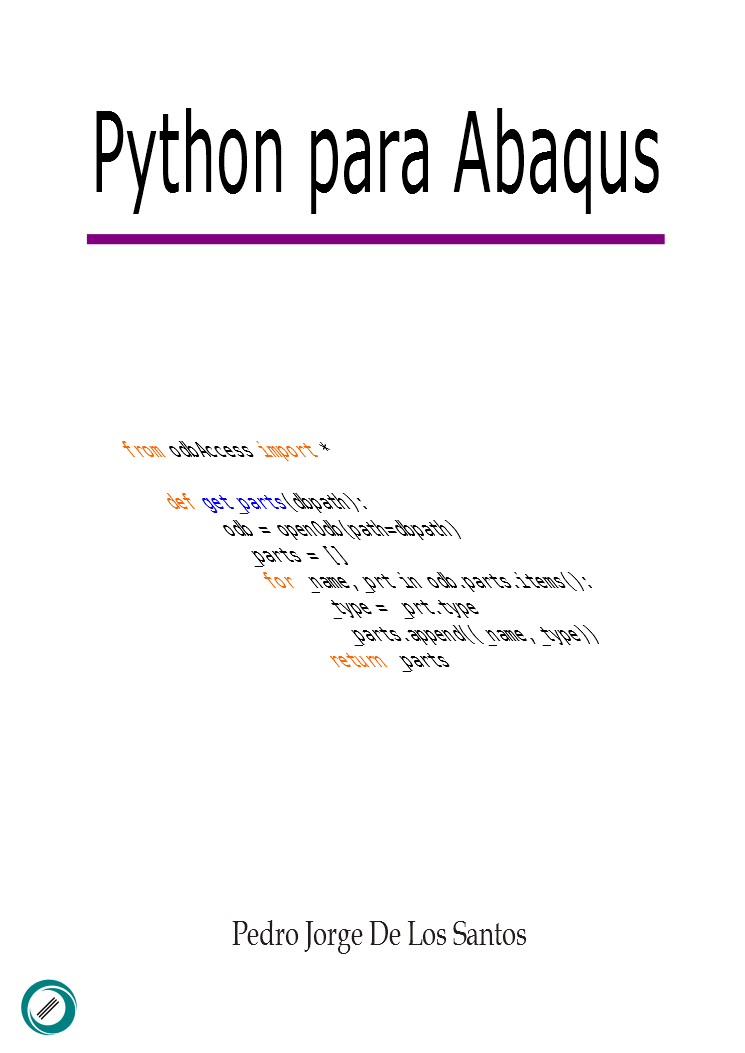
\includepdf{src/portada}
\maketitle
\tableofcontents

\chapter*{Acerca de...}

Estos apuntes de \textit{Python para Abaqus} han nacido con la finalidad de ayudar a usuarios 
hispanohablantes en el desarrollo de scripts en lenguaje Python para agilizar tareas 
de preprocesado o postprocesado en Abaqus.\\

Un poco a la par de este texto se ha desarrollado una pequeña librería de Python (PyQus) que puede 
ser utilizada para algunas tareas de postproceso de archivos de salida de Abaqus (ODB). Puede 
encontrar los códigos y la documentación correspondiente en el repositorio de GitHub 
\href{https://github.com/JorgeDeLosSantos/pyqus}{{\color{blue} PyQus}}\\


\texttt{Pedro Jorge De Los Santos}\\
\texttt{delossantosmfq@gmail.com}\\

\href{https://labdls.blogspot.mx}{
\includegraphics[scale=0.1]{src/ch0/blogger_logo.png}}
\href{https://www.youtube.com/user/lab2dls}{
\includegraphics[scale=0.1]{src/ch0/youtube_logo.png}}
\href{https://github.com/JorgeDeLosSantos}{
\includegraphics[scale=0.08]{src/ch0/github_logo.png}}
\href{https://www.linkedin.com/in/pjdlsl}{
\includegraphics[scale=0.1]{src/ch0/linkedin_logo.png}}
\href{https://plus.google.com/u/0/+pjdelossantos}{
\includegraphics[scale=0.1]{src/ch0/google_logo.png}}
\chapter{Fundamentos de Python}

Python es un lenguaje de programación desarrollado a finales de los 
80's y con sus primeras versiones liberadas en los albores de los 90's. Se caracteriza por ser interpretado, 
de tipado dinámico, multiparadigma y multiplataforma. Posee una licencia de código abierto (PSFL) 
desarrollada por la Python Software Foundation (PSF), de modo que el acceso al código fuente del proyecto 
está disponible para los desarrolladores. Lo anterior ha permitido, en gran medida, la proliferación 
de una comunidad sólida alrededor del mismo.\\

Es un lenguaje de propósito general, relativamente sencillo de aprender y con un potencial enorme. 
Sus aplicaciones pueden pasar desde un simple script para uso personal en las tareas comunes con 
el ordenador, el desarrollo web, la seguridad informática, y desde luego, las aplicaciones en el 
ámbito científico y de ingeniería.

\section{Tipos de datos}

\subsection{Enteros}

En matemáticas se clasifican como enteros aquellos números en el intervalo $ (-\infty,\infty) $, 
que no contienen una parte decimal o fraccionaria. Dadas las limitaciones de los ordenadores 
es evidente que no podrá representarse un entero demasiado "grande", generalmente el límite 
de representación es dado por las características del procesador.\\

En Python existen 2 tipos de enteros: el tipo entero ordinario (int) y el entero largo (long). 
La diferencia es precisamente el límite de representación de cada uno. Puede obtener información 
acerca del máximo entero tecleando lo siguiente en el intérprete de Python:

\begin{python}
	>>> import sys
	>>> max_int=sys.maxint
	>>> max_intl=sys.maxsize
\end{python}

Siendo max_int el entero ordinario máximo representado, generalmente este valor equivale a 
(2^31)-1. El valor de max_intl corresponde al máximo entero largo.\\

Para definir un tipo entero no hace falta declararlo de forma explícita, por ejemplo:

\begin{python}
	>>> a=1
	>>> b=100
	>>> type(a)
	<type 'int'>
	>>> type(b)
	<type 'int'>
	>>> c=-100
	>>> type(c)
	<type 'int'>
\end{python}

\subsection{De punto flotante}

Los números de punto flotante son aquellos que normalmente conocemos como números reales. 
En Python para que un valor numérico sea "reconocido" como real, debe utilizarse la función 
float o bien añadir la parte decimal del número, aun cuando esta sea nula:

\begin{python}
	>>> a=3
	>>> b=float(3)
	>>> c=3.0
	>>> type(a),type(b),type(c)
	(<type 'int'>, <type 'float'>, <type 'float'>)
\end{python}


\subsection{Booleanos}

También conocidos como valores lógicos, son un tipo de dato fundamental, cuyo valor sólo 
puede adquirir dos estados: verdadero y falso. Se utilizan comunmente para la toma de 
decisiones en conjunto con las estructuras de control de flujo. Las constantes booleanas 
en Python se nombran mediante True y False.\\

Por ejemplo, si comparamos dos números enteros cualesquiera para ver si son iguales:

\begin{python}
	>>> a=10
	>>> b=15
	>>> a==b
	False
	>>> a>b
	False
	>>> a<b
	True
\end{python}


\subsection{Cadenas de caracteres}


\subsection{Listas}


\subsection{Tuplas}


\subsection{Diccionarios}



\section{Estructuras de control}

\subsection{Sentencia if}

La sentencia if es una estructura de control flujo simple, utilizada para la toma 
de decisiones en el curso de ejecución que sigue el programa. En casi todos los algoritmos 
existen porciones de código que sólo deben ejecutarse cuando se cumpla una condición 
establecida, es ahí donde la sentencia if tiene su utilidad. Vea el ejemplo dado 
a continuación:

\begin{python}
a = 10
	if a > 0:
	    print "Número positivo"
\end{python}

Veamos: primero se define una variable {\bf a} con valor 10, posteriormente se hace la 
comprobación que si {\bf a} es mayor a cero, lo cual implicaría imprimir en pantalla 
un mensaje, de lo contrario no se realizará acción alguna. Para el ejemplo mostrado, 
puesto que {\bf a} es 10, entonces es un número positivo, y por ende se ejecutará la 
porción de código incluido en la sentencia if.\\

En muchas situaciones la sentencia if se utiliza en conjunto con la sentencia 
complementaria else, para formar una bifurcación doble, que permite seleccionar 
una opción especificada o bien otra por default. A manera de ejemplo vamos a desarrollar 
un programa que determinará si un número ingresado es par o impar:

\begin{python}
	n = input("n = ")
	if (-1)**n == 1:
	    print "Par"
	else:
	    print "Impar"
\end{python}

Si la condición propuesta se cumple entonces se ejecutará el bloque incluido dentro de la 
sentencia if, en cualquier otro caso se ejecutará el bloque definido por la cláusula else.\\

Además de las anteriores, existe otra forma más general definida por las sentencias  
if-elif-else cuya estructura general es:

\begin{python}
	if cond1:
	    # ... 
	elif cond2:
	    # ...
	elif cond3:
	    # ...
	.
	.
	.
	elif condN:
	    # ...
	else:
	    # ...
\end{python}

La anterior es un tipo de bifurcación múltiple, que permite seleccionar entre varias 
condiciones definidas en la cláusula if y en las subsecuentes elif, y una 
opción por defecto establecida en la cláusula else. Un ejemplo: 

\begin{python}
	n = input("n = ")
	if n>0:
	    print "Positivo"
	elif n<0:
	    print "Negativo"
	else:
	    print "Cero"
\end{python}


\subsection{Bucle for}


\subsection{Bucle while}

\chapter{Geometrías, secciones y materiales}

\chapter{Postprocesando archivos ODB}

\section{Procesando información básica}

\subsection{Partes}

Las partes o geometrías son las entidades básicas en Abaqus, y a partir las cuales se construye el ensamble 
o modelo. Las partes pueden ser bidimensionales o tridimensionales, deformables o rígidas, dependiendo 
de las características del cuerpo físico a representar.\\

Para leer información acerca de las partes incluidas en un archivo ODB, debemos primeramente leer el archivo 
y enseguida acceder al diccionario \texttt{parts}.\\

En el siguiente código se imprimen en consola todas las partes que contiene el archivo \textit{ejemplo.odb}, 
y adicionalmente se imprime el tipo de la parte en cuestión (Deformable, Analítica,...).

\begin{python}
from odbAccess import openOdb

dbpath = "ejemplo.odb"
odb = openOdb(path=dbpath)
for _name,_prt in odb.parts.items():
	print _name, _prt.type
\end{python}

Pero claro, siempre que sea posible es mejor escribir código que pueda ser reutilizado, en forma de funciones y/o clases 
que puedan almacenarse en módulos y posteriormente importarse en un script donde sean utilizadas.\\

En el siguiente código se define una función {\tt get\_parts} que básicamente lee la información de las partes que 
componen el archivo de salida, devolviendo una lista de tuplas con los nombres y tipos de las partes.

\begin{python}
from odbAccess import *

def get_parts(dbpath):
	odb = openOdb(path=dbpath)
	_parts = []
	for _name,_prt in odb.parts.items():
		_type = _prt.type
		_parts.append((_name,_type))
	return _parts
\end{python}


\subsection{Secciones}

\subsection{Materiales}

\subsection{Pasos de carga}

\subsection{Interacciones}

\subsection{Instancias}

%\printindex

\end{document}
